\section{Problem Statement and Model}
This section further elaborates on the problem and how it is modelled.
\subsection{Network}
The actual problem domain is a network modelled as a directed graph $N = (V,L)$, with no limits to the number of existing nodes.
In reality are the nodes contained in $V$ some kind of hardware on that virtual network functions can be started.
The links $L$ represent the physical connections between these hardware elements.
Figure \ref{fig:networkexample} shows a small example of such a network.
The network can also have any number of ingress and egress nodes.
In the example, the network has two ingress and one egress node ($A,C,B\in V$).
The connections ${x}_{1}, {x}_{2}, {y}_{1} \in L$ describe the ingress and egress connection of the system.
These connections represent an infinite number of possible connections to nodes that request a service or receive the result of a service process, that is why they are substituted as simple arrows in the figure.
Each node can be ingress and egress node at the same time, meaning it can have an ingress and egress connection.
All the incoming traffic flows over the connections ${x}_{n}$ and over the connections ${y}_{n}$, where all outgoing traffic leaves the system.

\begin{figure}[H]
	\centering
	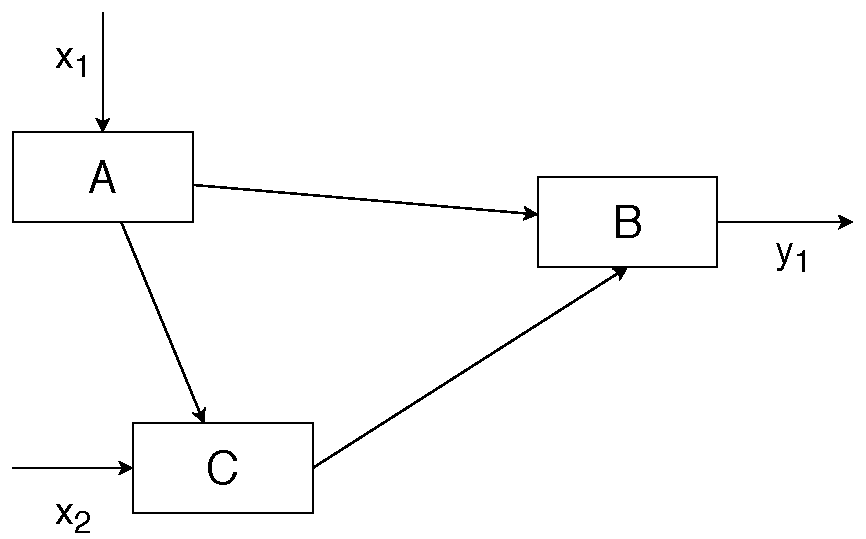
\includegraphics[width=0.6\linewidth]{Pictures/NetworkExample}
	\caption{Example for a network with two ingress and one egress node.}
	\label{fig:networkexample}
\end{figure}

\subsection{Services}
Services are modeled with directed acyclic graphs $S = ({V}_{S},{L}_{S})$.
Each node in ${V}_{S}$ represents a function (Virtual Network Function), which gives the result to the next node in the graph or outputs it from the network.
The function nodes can be placed at any node of the network $N$.
One restriction is the fact that the connection from ${L}_{S}$ has to be mapped to the connections $L$ of $N$.
Figure \ref{fig:networService} displays an example of this.
The service with two VNFs, $v_{S1},v_{S1} \in V_{S}$, is placed in the network with $v_{S1}$ placed at $A$ and $v_{S2}$ placed at $B$.
Placing $v_{S1}$ at $C$ and $v_{S2}$ at $A$ would not be possible since there is no path from $C$ to $A$ and the necessary connection of the service could not have been mapped to the network.

\begin{figure}
	\centering
	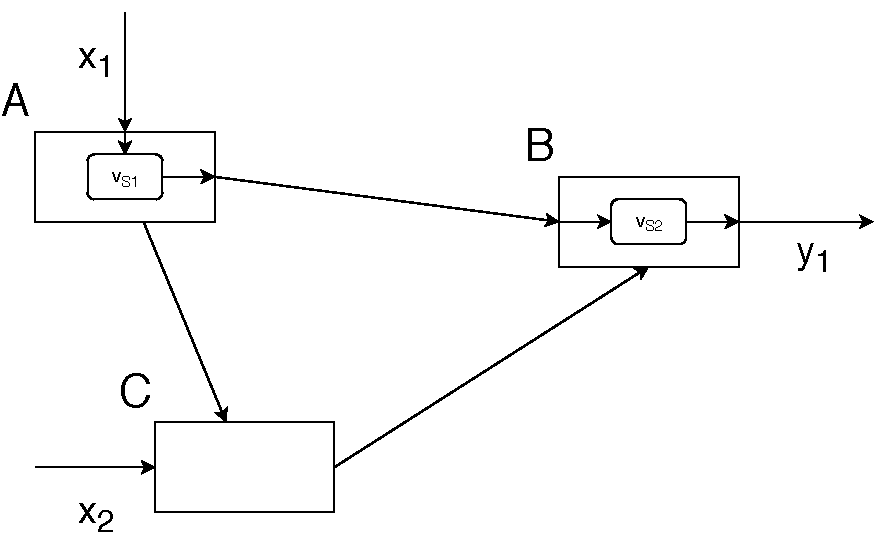
\includegraphics[width=0.6\linewidth]{Pictures/NetworkExampleWithService}
	\caption{Previous network with an example service included.}
	\label{fig:networService}
\end{figure}

\subsection{Traffic}
Now coming back to the actual problem of predicting the network traffic.
The relevant parts for the problem of this thesis are the incoming traffic and the nodes where the traffic arrives.
The structure, the internal traffic (between ingress and egress nodes) and the output traffic of the network has no relevance for this problem solution.
So the actual feature that this thesis predicts is the traffic for each service at each ingress node.
The traffic $x_{n}$ splits up into the traffic for the different services.

What is also important for the prediction of the traffic apart from the system itself are additional information about the traffic.
One of the most important examples is the date and time of the incoming traffic.
Since at different days and time of day the traffic changes drastically.